\chapter[Matematická kryptografie]{B4M01MKR \\[1ex]\Large{Symetrická a asymetrická kryptografie. Základní kryptosystémy. Faktorisace čísel. Hashování}}

\section{Symetrická a asymetrická kryptografie}
Symetrická a asymetrická kryptografie se liší vlastnostmi a způsobem použití
klíčů. Zatímco v symetrické kryptografii používají obě komunikující strany
stejný klíč, u asymetrické kryptografie jsou klíče dva: soukromý klíč (často
značený $d$), a veřejný klíč (často značený $e$).

Symetrická kryptografie je rychlejší a proto se používá pro většinu komunikace,
ale vyžaduje bezpečnou výměnu klíče. Asymetrická kryptografie je pomalejší, a
podle použití klíčů umožňuje dvě věci:
\begin{itemize}
\item Kdokoliv může zašifrovat zprávu veřejným klíčem, a zprávu si pak může
přečíst jen ten, komu je určena (majitel soukromého klíče)
\item Majitel klíče pošle zprávu a k ní hash zašifrovaný soukromým klíčem.
Takovou zprávu si může kdokoliv přečíst, ale zprávu nelze zfalšovat (je jasné,
že autorem může být jedině majitel klíče).
\end{itemize}

Díky tomu mohla vzniknout hierarchie certifikačních autorit a certifikátů.
Uživatel může ověřit (podle certifikační autority, které věří), že server na
druhé straně komunikace se za nikoho nevydává, a skutečně jde třeba o webovou
stránku banky. S použitím asymetrické kryptografie si uživatel se serverem
vymění hesla a dál mohou používat rychlejší symetrickou kryptografii.

\section{Matematika používaná v kryptografii}
\subsection{Dělitelnost, modulo, rovnice}

Základní věta aritmetiky: Každé přirozené číslo $n$ jde zapsat jako jednoznačný
součin prvočísel, kde \textbf{prvočíslo} je číslo, které je dělitelné jen
jedničkou a sebou samým.

\subsubsection{Počítání modulo}

\textbf{Dělení se zbytkem}: $\forall a, b \in \mathbb{Z}, a, b > 0, \exists q, r
\in \mathbb{Z},$ že $ a = qb + r$, a přitom $0 \leq r \le b$, a $q, r$ jsou
jednoznačné. Když je $r$ (zbytek) nulový, řekneme, že $a$ je dělitelné $b$ nebo
že $b$ dělí $a$, značíme $b \mid a$. Relace dělitelnosti na $\mathbb{Z}$ je
reflexivní, tranzitivní a antisymetrická, dá se znázornit Hasseho diagramem
(Obrázek \ref{fig:hasse}).

\begin{figure}[ht!]
\label{fig:hasse}
\centering
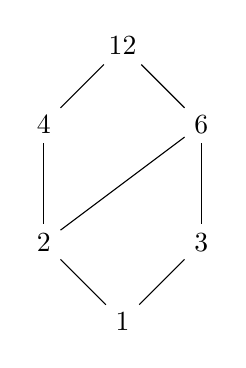
\begin{tikzpicture}
    \node (12) at (0,0) {12}; \node (4) at (-1, -1) {4}; \node (6) at (1, -1)
    {6}; \node (2) at (-1, -2.5) {2}; \node (3) at (1, -2.5) {3}; \node (1) at
    (0, -3.5) {1} ;

    \path  (12) edge node {} (4); \path  (12) edge node {} (6); \path  (6) edge
    node {} (2); \path  (6) edge node {} (3); \path  (4) edge node {} (2); \path
    (1) edge node {} (2); \path  (1) edge node {} (3);
\end{tikzpicture}
\caption{Hasseho diagram pro číslo 12}
\end{figure}

\textbf{Největší společný dělitel (GCD)} dvou čísel $a, b$ (značíme $gcd(a,b)$)
je takové číslo $d$, kde:
\begin{itemize}
\item $d \mid a \wedge d \mid b$
\item $d$ je dělitelné všemi společnými děliteli obou čísel
\item $d \geq 0$
\end{itemize}
V Hasseho diagramu najdeme GCD dvou čísel jako první číslo, ve kterém se můžeme
sejít při cestě dolů - pro čísla 4 a 6 jde o číslo 2.

\textbf{Nejmenší společný násobek (LCM)} čísel $a, b$ (značíme $lcm(a, b)$) je
nejmenší takové $d$, které je dělitelné číslem $a$ a zároveň je dělitelné číslem
$b$. V Hasseho diagramu najdeme LCM jako první číslo, ve kterém se můžeme sejít
při cestě nahoru - pro čísla 3 a 4 je LCM 12.

Máme nějaké $n \in \mathbb{N}$, pak čísla $a, b \in \mathbb{Z}$ jsou
\textbf{kongruentní modulo} $n$, pokud $n \mid (b-a)$. Kongruence se značí $a
\equiv b\mod n$, je to ekvivalence a rozdělí celá čísla na $n$ tříd, kde všechny
prvky ve třídě mají stejný zbytek po dělení číslem $n$. Přirozená čísla
rozdělená na třídy ekvivalence podle $n$ značíme $\mathbb{Z}_n$. Relace
kongruence je zachovaná při sčítání i násobení.

Například můžeme celá čísla rodělit podle $\mathbb{Z}_4$:
\begin{itemize}
\item ${-4, 0, 4, ...} \equiv  0$
\item ${-3, 1, 5, ...} \equiv  1$
\item ${-2, 2, 6, ...} \equiv  2$
\item ${-1, 3, 7, ...} \equiv  3$
\end{itemize}

A kongruence je zachovaná i při násobení a sčítání:

\begin{itemize}
\item $-4 \times 3 = -12 = 0$, nebo $-4 \times 3 = 0 \times 3 = 0$ 
\item $-4 + 3 = -1 = 3$, nebo $-4 + 3 = 0 + 3 = 3$ 
\end{itemize}

\subsubsection{Euklidův algoritmus}
\textbf{Euklidův algoritmus} umožňuje v lineárním čase najít $gcd(a,b)$. Dělá to
tak, že rozkládá $a$ jako $a = qb + r$, a dokud je zbytek $r$ nenulový,
rekurzivně spouští $gcd(b,r)$. Výhodné je použít místo tohoto postupu výpočet
přes úpravy matic, kde dostaneme navíc koeficienty pro Bezoutovu větu.

\begin{exercise}

\textbf{Př.:} Najděte $gcd(260, 84)$ s použitím Euklidova aloritmu.

\begin{center}
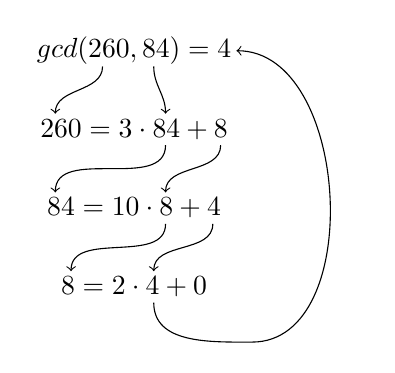
\begin{tikzpicture}; \node (A) at (0, 0) {$gcd(260, 84) = 4$}; \node (B) at (0,
    -1) {$260 = 3 \cdot 84 + 8$}; \node (C) at (0, -2) {$84 = 10 \cdot 8 + 4$};
    \node (D) at (0, -3) {$8 = 2 \cdot 4 + 0$};
    
    \draw[->](-0.4,-0.2) to[out=270,in=90] (-1,-0.8); \draw[->] (0.25,-0.2)
   	 to[out=270,in=90] (0.4,-0.8);
   	 
    \draw[->](0.4,-1.2) to[out=270,in=90] (-1,-1.8); \draw[->] (1.1,-1.2)
   	 to[out=270,in=90] (0.4,-1.8);
   	 
    \draw[->](0.4,-2.2) to[out=270,in=90] (-0.8,-2.8); \draw[->] (1,-2.2)
   	 to[out=270,in=90] (0.25,-2.8);
   	 
   	 \draw (0.25,-3.2) to[out=270,in=180] (1.5, -3.7); \draw[->] (1.5, -3.7)
   	 to[out=0,in=0] (1.3, 0);
\end{tikzpicture}
\end{center}

Jakmile získáme $r = 0$, tak víme, že hodnota GCD je uložena v $b$. V tomto
případě $gcd(260, 84) = 4$.

\end{exercise}

\begin{exercise}
\textbf{Př.:} Najděte $gcd(260, 84)$ maticově.

\[ \left( \begin{array}{cc|c}
1 & 0 & 260\\
0 & 1 & 84 \end{array} \right)
%
\sim
%
\left( \begin{array}{cc|c}
1 & -3 & 8\\
0 & 1 & 84 \end{array} \right)
%
\sim
%
\left( \begin{array}{cc|c}
1 & -3 & 8\\
-10 & 31 & 4 \end{array} \right)
%
\sim
%
\left( \begin{array}{cc|c}
21 & -65 & 0\\
-10 & 31 & 4 \end{array} \right) \]

Maticové řešení je podrobněji popsané níže u diofantických rovnic. Kromě toho,
že jsme našli řešení, máme i jiné užitečné vztahy, a sice vyjádření nuly: $21
\cdot 260 - 65 \cdot 84 = 0$ a vyjádření GCD: $-10 \cdot 260 + 31 \cdot 84 = 4$.
Maticový výpočet se hodí, když hledáme GCD více čísel najednou:

\[ \left( \begin{array}{ccc|c}
1 & 0 & 0 & 90\\
0 & 1 & 0 &  78\\
0 & 0 & 1 &  72 \end{array} \right)
%
\sim
%
\left( \begin{array}{ccc|c}
1 & 0 & -1 & 18\\
0 & 1 & -1 &  6\\
0 & 0 & 1 &  72 \end{array} \right)
%
\sim
%
\left( \begin{array}{ccc|c}
1 & -3 & 2 & 0\\
0 & 1 & -1 &  6\\
0 & -12 & 13 &  0 \end{array} \right) \]

\[ \left( \begin{array}{ccc|c}
1 & 0 & 0 & 70\\
0 & 1 & 0 &  110\\
0 & 0 & 1 &  154 \end{array} \right)
%
\sim
%
\left( \begin{array}{ccc|c}
1 & 0 & 0 & 70\\
-1 & 1 & 0 &  40\\
-2 & 0 & 1 &  14 \end{array} \right)
%
\sim
%
\left( \begin{array}{ccc|c}
11 & 0 & -5 & 0\\
5 & 1 & -3 &  -2\\
-2 & 0 & 1 &  14 \end{array} \right)
%
\sim
%
\left( \begin{array}{ccc|c}
11 & 0 & -5 & 0\\
-5 & -1 & 3 &  2\\
33 & 7 & -20 &  0 \end{array} \right) \]
\end{exercise}

\subsubsection{Bezoutova věta}
\textbf{Bezoutova věta} říká, že největší společný dělitel jde zapsat jako vztah
$a,b$, tedy: $gcd(a, b) = sa + tb$, kde $s,t$ jsou celá čísla.

\subsubsection{Diofantické rovnice}
\textbf{Diofantická rovnice} je rovnice ve tvaru $ax + by = c$, kde $a,b,c \in
\mathbb{Z}$. Diofantická rovnice má řešení, právě když $gcd(a,b) \mid c$. Řešení
má partikulární a homogenní část.

\begin{exercise}
    
\textbf{Př.:} V $\mathbb{Z}_{45}$ řešte rovnici $12x = 6$.

Rovnici si nejprve převedeme na diofantickou, tj dostaneme $12x + 45y = 6$.
Vyrobíme si jednotkovou matici o dvou sloupcích, kde první sloupec odpovídá
neznámé $x$ a druhý sloupec neznámé $y$. Příslušné hodnoty v rovnici napíšeme do
pravého sloupce a matici upravíme.
\[ \left( \begin{array}{cc|c}
1 & 0 & 12\\
0 & 1 & 45 \end{array} \right)
%
\sim
%
\left( \begin{array}{cc|c}
1 & 0 & 12\\
-4 & 1 & -3 \end{array} \right)
%
\sim
%
\left( \begin{array}{cc|c}
-15 & 4 & 0\\
-4 & 1 & -3 \end{array} \right) \] Úpravy skončí, když se v pravém sloupci
objeví nula. Druhá hodnota je největší společný dělitel čísel 12 a 45, po
přenásobení řádku $-1$ vidíme, že $gcd(12,45)=3$. Protože $3 \mid 6$, bude mít
diofantická rovnice řešení.

Máme homogenní řešení $12\times(-15) + 45\times 4 = 0$ a partikulární řešení
$12\times4 + 45\times(-1) = 3$. Druhou rovnici ale musíme vynásobit dvěma,
abychom dostali na pravé straně 6 (odtud požadavek, aby $3\mid6$), tím dostaneme
partikulární řešení $12\times8 + 45\times(-2) = 6$. Řešení se zapisuje ve tvaru
$(x,y) = (x_p,y_p) + k(x_0,y_0)$, a řešení diofantické rovnice je $(x,y) = (8,
-2) + k(-15,4)$. V zadání jsme ale měli řešit pouze rovnici pro $x$, a tak
výsledek je $x = 8 - 15k$.
\end{exercise}

\subsection{Grupy}
Máme množinu $A$ a operaci $\cdot$~. Dvojice $(A,\cdot)$ je grupa, pokud:
\begin{itemize}
\item Platí asociativita, tj $x\cdot(y\cdot z) = (x\cdot y)\cdot z$
\item Existuje neutrální prvek $e \in A$ (jednotka), pro který platí, že
$\forall x \in A: e\cdot x = x = x \cdot e$.
\item Všechny prvky mají inverze, tj $\forall x ~\exists y: x\cdot y = e = y
\cdot x$.
\end{itemize}
Řekneme, že $(A,\cdot)$ je Abelova grupa, když je navíc operace $\cdot$
komutativní, tedy $x\cdot y = y \cdot x$. Dvojice $(\mathbb{Z}, +)$,
$(\mathbb{R}^+, \times)$,  $(\mathbb{Z}_n, +)$ jsou grupy. $(\mathbb{Z}_n^*,
\times)$, kde $\mathbb{Z}_n^*$ je podmnožina prvků ze $\mathbb{Z}_n$
nesoudělných s $n$, je taky grupa.

\textbf{Řád grupy} je počet prvků v $A$. Grupy mohou být konečné i nekonečné.

V grupách $\mathbb{Z}_n^*$ jsou všechna čísla menší než $n$, která jsou s $n$
nesoudělná. Počet nesoudělných čísel, a tedy i řád grupy, vyjadřuje
\textbf{Eulerova funkce} $\varphi(n)$.
\begin{itemize}
\item $\varphi(p) = p-1$ pro prvočíslo $p$.
\item $\varphi(p^k) = p^k - p^{k-1} = p^{k-1}(p-1)$ pro $k$-tou mocninu
prvočísla $p$.
\item $\varphi(n\cdot m) = \varphi(n)\cdot\varphi(m)$ pro nesoudělná čísla
$m,n$.
\end{itemize}

Nejmenší $m$ takové, že $\forall a \in G: a^m = 1$ se nazývá \textbf{exponent
grupy}. Exponent grupy $\mathbb{Z}_n^*$ lze spočítat \textbf{Carmichaelovou
funkcí} $\lambda(n)$.
\begin{itemize}
\item $\lambda(\prod_{i=1}^r p_i^{e_i}) = lcm\{\lambda(p_1^{e_1}), \ldots,
\lambda(p_r^{e_r})\}$ pro složené číslo.
\item $\lambda(p^e) = \varphi(p^e) = p^e - p^{e-1} = p^{e-1}(p-1)$ pro $e$-tou
mocninu prvočísla $p$, kde $p > 2$.
\item $\lambda(2^e) = \frac{\varphi(2^e)}{2} = 2^{e - 2}$ pro mocninu dvojky,
kde $e \geq 3$.
\item $\lambda(4) = 2$
\item $\lambda(2) = 1$
\end{itemize}

\subsubsection{Cyklické grupy}

Nechť $(G,\cdot)$ je grupa s neutrálem 1, $a \in G$. Nejmenší $r \in \mathbb{N}$
takové, že $a^r = 1$ v $G$ se nazývá \textbf{řád prvku} $a$, značí se $r(a)$.
Pokud takové číslo neexistuje, je řád nekonečný.

Pro prvek $a \in G$ je množina $P = \{a^i~|~i = 1 \ldots r(a)\}$
\textbf{cyklickou podgrupou} grupy $G$. Cyklickou podgrupu generovanou prvkem
$a$ značíme $\langle a \rangle$. Pokud pro nějaký prvek $a \in G$ platí $\langle
a \rangle  = G$, pak řekneme, že grupa $G$ je \textbf{cyklická} a prvek $a$ je
její \textbf{generátor}.

Grupy $(\mathbb{Z}, +)$ a $(\mathbb{Z}_n, +)$ jsou cyklické a jejich generátorem
je např. prvek 1. Grupy $(\mathbb{Z}_n^*, \times)$ jsou cyklické pro $n$
prvočíslo, mocninu prvočísla, nebo $n$ ve tvaru $2p^e$ pro liché prvočíslo $p$.

Cyklické grupy jsou specifické tím, že mají jasné velikosti podgrup a od každé
velikosti existuje jen jedna podgrupa.

\subsection{Euler-Fermatova věta}
Nechť $(G,\cdot)$ je konečná grupa s neutrálem 1. Pak $\forall a \in G: a^{|G|}
= a\cdot a\cdot a\cdots a = 1$ v $G$.

To nám říká, že když umocníme na velikost grupy, dostaneme jednotku.
Euler-Fermatova věta se používá při počítání velkých mocnin, protože umožňuje
zmenšit exponent.

\subsection{Algoritmus opakovaných čtverců}

Algoritmus opakovaných čtverců taky zrychluje počítání mocnin. Fungování je
nejlépe vidět na příkladu.

\begin{exercise}
\textbf{Př.:} Spočítejte $5^{17}$ v $\mathbb{Z}_{27}$.
\begin{enumerate}
\item Exponent napíšeme jako binární číslo:\\ $17 = 16 + 1 = 10001_{bin}$
\item Do mezer mezi cifry vložíme znak $S$, nuly smažeme, jedničky nahradíme
znakem $X$:\\ $10001 = 1S0S0S0S1 = 1SSSS1 = XSSSSX$.
\item Začneme s číslem 1 a postupně zpracováváme znaky $S$ a $X$. Po přečtení
znaku $S$ mezivýsledek umocníme na druhou, po přečtení znaku $X$ mezivýsledek
vynásobíme základem. Přitom pořád si mezivýsledek udržujeme v modulu $n$:\\
$1XSSSSX \rightarrow 5SSSSX \rightarrow 25SSSX = -2SSSX \rightarrow 4SSX
\rightarrow 16SX \rightarrow 256X = 13X \rightarrow 65 = 11$ v
$\mathbb{Z}_{27}$.
\end{enumerate}
\end{exercise}

\subsection{Čínská věta o zbytcích}
Díky čínské větě umíme řešit soustavy rovnic. Mějme po dvou nesoudělná přirozená
čísla $n_1, \ldots, n_k$ a k nim libovolná přirozená čísla $a_1,\ldots,a_k$. Pak
soustava rovnic $x_i \equiv a_i \mod n_i, i = 1,\ldots,k$ má právě jedno řešení
modulo $n = \prod_{i=1}^{k}n_i$.

Řešení se najde tak, že pro každou rovnici najdeme takové $q_i$, aby platil
vztah $q_i \equiv 1 \mod n_i$ a zároveň $q_i \equiv 0 \mod n_j, j \neq i$ (tedy
$q_i$ je nulové ve všech modulech vyjma svého vlastního, kde má hodnotu jedna).

Takové $q_i$ můžeme najít tak, že vynásobíme všechny moduly (vyjma $n_i$),
výsledek označme $m_i$, a najdeme nějaké $t_i$ tak, aby $m_it_i \equiv 1 \mod
n_i$. Tato soustava určitě bude mít řešení, protože $n_i$ jsou nesoudělná.
Tím získáme $q_i = m_it_i \mod n$.

Řešení soustavy pak je $x = \sum_{i=1}^{k}q_ia_i$.

\begin{exercise}
\textbf{Př.:} Řešte soustavu: $x \equiv 2 \mod 4$, $x \equiv 0 \mod 5$, $x
\equiv 1 \mod 9$, $x \equiv 2 \mod 11$.

Spočítáme koeficient $q$ pro modul 4. $q_4 = 5\cdot9\cdot11\cdot t = 495t$.
Chceme, aby $495t \equiv 1 \mod 4$, což si můžeme ještě upravit na $3t \equiv 1
\mod 4$. Vidíme, že vhodné $t$ je 3, protože $3\times 3 = 9 \equiv 1 \mod 4$.
Dosazením hodnoty $t$ dostaneme $q_4 = 495t = 495 \times 3 = 1485$. Obdobně
dostaneme $q_5 = 396$, $q_9 = 1540$, $q_{11} = 540$.

Z koeficientů dostaneme výsledek: $x = 2q_4 + 0q_5 + 1q_9 + 2q_{11} = 2970 + 0 +
1540 + 540 = 5590$. Ale my pracujeme modulo $n = 4\cdot5\cdot9\cdot11 = 1980$,
proto je výsledek $x = 5590 \equiv 3610 \equiv 1630 \mod 1980$.

\end{exercise}

\section{Generování prvočísel}
Generování prvočísel zjednodušeně probíhá tak, že se (chytře) generují čísla, a
následně se ověřuje, jestli vzniklo prvočíslo. Testy prvočíselnosti můžeme dělat
deterministicky nebo pravděpodobnostně. Deterministické testy zmíníme jen
okrajově:

\begin{itemize}
\item \textbf{Hrubou silou}: Dělíme $n$ všemi (prvo)čísly až do $\sqrt{n}$ a tím
vyloučíme dělitelnost. Složitost takového postupu je $O(2^{0.5\cdot len(n)}\cdot
len(n))$
\item \textbf{Agrawal, Kayal, Saxena (AKS)}:  test prvočíselnosti je sice
polynomiální a deterministický, ale jeho složitost je $O(len(n)^{10.5 + o(1)})$
\end{itemize}

Pravděpodobnostní testy mají jednostrannou chybu. Pokud odpoví, že číslo je
\texttt{složené}, je to vždy pravda. Odpověď \texttt{prvočíslo} ale správná být
nemusí - mohlo se stát, že test důkaz o složenosti "přehlédl". Ve vstupu testu
je testované číslo a nějaký svědek. Na základě jednoho svědka algoritmus
rozhodne. Pro získání požadované spolehlivosti se test několikrát opakuje s
různými svědky.

\subsection{Fermatův test}
Fermatův test zavádí pro testované $n$ množinu svědků prvočíselnosti $K_n$, ve
které jsou ty prvky, které po umocnění na $n-1$ vrátí jedničku. To vychází z toho,
že dle Euler-Fermatovy věty platí $a^{|G|} = 1$, a pokud je $n$ opravdu prvočíslo,
tak musí platit $a^{|G|} = a^{\varphi(n)} = a^{n-1} = 1 \mod n$.

Pokud je $n$ prvočíslo, pak $K_n$ je shodná s $\mathbb{Z}_n^*$ - to znamená, že 
množina svědků je stejná jako množina, ze které bereme, a test vždycky projde.
Pokud $n$ není prvočíslo, pak se rozdělí $\mathbb{Z}_n^*$ na třídy (podgrupy). Počet tříd
$k$ nutně dělí velikost grupy.
\begin{itemize}
\item Pro $k = 1$ nastává výjimečná situace, totiž že $|\mathbb{Z}_n^*| =
|K_n|$. Takové složené $n$ se nazývá Carmichaelovo a platí pro něj, že $a^{n-1}
= 1 \mod n$ pro libovolné $a$. Fermatův test nedokáže rozpoznat Carmichaelova
čísla jako složená.
\item Pro $k \geq 2$ platí, že  $|K_n| = \frac{1}{k}|\mathbb{Z}_n^*|$.  Obecně
můžeme říct, že $|K_n| \leq \frac{1}{2}|\mathbb{Z}_n^*|$, ale to je hrubý odhad,
častěji bude $K_n$ daleko menší. Tohle nám říká, že jen $\frac{1}{k}$ ze zkoušených 
čísel budou svědci, tedy bude to falešně vypadat, že máme prvočíslo. V $\frac{k-1}{k}$
případech nám mocnění nevyjde a budeme moci $n$ označit za složené.
\end{itemize}

Fermatův test bere na vstupu testované číslo $n$ a svědka $a$.
\begin{verbatim}
fermat-test(n, a):
    b = pow(a, n-1) % n
    if b == 1:
        return "asi prvočíslo"
    else:
        return "určitě složené"
\end{verbatim}

\begin{exercise}
\textbf{Př.:} Fermatovým testem ověřte, zda 21 je prvočíslo. Použijte svědky 8,
6 a 2. 
\begin{itemize}
\item \texttt{fermat-test(21, 8) = "asi prvočíslo"}, protože $8^{20} = \cdots =
1 \mod 21$.  Pravděpodobnost chyby je nejvýš 1/2. Pokud bychom si to spočítali
(našli řešení $x^{20} = 1$), uvidíme, že takové $x$ jsou čtyři (1, 8, 13, 20) a
zabírají pětinu z celkových 20ti prvků. Pravděpodobnost omylu testu je tedy
daleko nižší, a to 1/5.
\item \texttt{fermat-test(21, 6) = "složené"}, protože $6^{20} = \cdots = 15
\neq 1 \mod 21$. Navíc když spočítáme gcd(21, 6) = 3, našli jsme jeden z
faktorů.
\item \texttt{fermat-test(21, 2) = "složené"}, protože $6^{20} = \cdots = 4\neq
1 \mod 21$. V tomto případě ale gcd(21, 2) = 1, takže nám to v hledání faktorů
nepomohlo.
\end{itemize}
\end{exercise}

\subsection{Miller Rabinův test}
Millerův test je složitější a přísnější než Fermatův v tom, že kromě výsledku
výpočtu sleduje i jeho průběh. Využívá toho, že pokud je $p$ prvočíslo, pak má
rovnice $a^2 = 1 \mod p$ pouze dvě řešení, a to $\pm 1$. To znamená, že
nenajdeme žádnou netriviální odmocninu (triviální odmocnina jedničky je mínus
jednička).

Miller Rabinův test zavádí množinu svědků $L_n$, která vybírá z $K_n$ jen ty
prvky, které při výpočtu prochází přes netriviální odmocninu z jedné. $L_n = \{a
\in \mathbb{Z}_n^*, a^{n-1} = 1, \text{a když } a^{t2^j} = 1, \text{pak }
a^{t2^{j-1}} = \pm 1 \text{ pro } \forall 1 \leq j \leq h \}$.

Máme liché testované číslo $n$ a rozložíme si $n-1 = t \cdot 2^h$ pro nějaké
liché $t$. V Miller Rabinově testu se svědci taky mocní na $n-1$ jako ve
Fermatově testu, ale mocní se postupně podle rozkladu a pozorují se
mezivýsledky.

\begin{exercise}
\textbf{Př.:} Miller Rabinovým testem ověřte, zda 21 je prvočíslo. Použijte
svědka 8.

$$n = 21, n-1 = 20 = 5 \cdot 4  = 5 \cdot 2^2$$
$$ 8 \xrightarrow{\text{mocníme na 5}} 8 \xrightarrow{\text{mocníme na 2}} 64 =
1 \xrightarrow{\text{mocníme na 2}} 1$$

V průběhu výpočtu jsme našli netriviální odmocninu jedné, a sice $8^2 = 64 = 1
\mod 21$ ($\sqrt{1} = 8$), a dle Miller Rabinova testu o prvočíslo nejde. Díky
netriviální odmocnině můžeme faktorizovat: gcd(8+1, 21) = 3, gcd(8-1, 21) = 7.
\end{exercise}


\section{Těžké matematické problémy}
\subsection{Faktorizace čísel}
Úloha faktorizace je složitá - snažíme se najít prvočíselný rozklad daného čísla
$n$. Mohli bychom zkoušet dělit čísly až do $\sqrt{n}$, ale takové dělení by
bylo pomalé (exponenciální). Rychleji se dá faktorizovat, pokud o $n$ něco víme,
a nebo použitím SubExponenciálního faktorizačního algoritmu (SEF).

\subsubsection{Faktorizace, když víme něco navíc}

Faktorizovat \textit{lépe} se dá se znalostí násobku $\lambda(n)$. O exponentu grupy
platí, že každý prvek grupy umocněný na exponent grupy je jedna, proto to bude
platit i o násobku exponentu grupy. Faktorizujeme tak, že najdeme netriviální
odmocninu z jedné, tj $c^2 = 1$. Jiné zjednodušení využívá znalosti $\varphi(n)
= p \cdot q$.

\begin{exercise}
\textbf{Př.:} Faktorizujte číslo 187, o kterém víte, že je součinem dvou
prvočísel a $\varphi(187) = 160$.

Označíme si použitá prvočísla jako $p$ a $q$. Jejich součin pak je $n = p \cdot
q = 187$. Obdobně vyjádříme $\varphi(n) = 160 = (p-1)(q-1) = pq - p - q + 1 = n
- p - q + 1 = 187 - p - q + 1$. Dalšími úpravami dostaneme vztah pro $p = 28 -
q$ (vztah pro $q$ by byl obdobný). Toto dosadíme do vztahu $n = p\cdot q$ a
dostaneme kvadratickou rovnici $q^2 - 28q + 187 = 0$, která má dvě řešení 11 a
17.
\end{exercise}

\begin{exercise}
\textbf{Př.:} Faktorizujte číslo 1771, znáte-li $\varphi(1771) = 1320$.

Rozdělíme si $\varphi(n) = 1320 = 165 \cdot 2 \cdot 2 \cdot 2$ podobně jako při
Miller Rabinově testu, a pokusíme se najít netriviální odmocninu jedné. Zvolme
$a = 5$.

$$ 5 \xrightarrow{\text{mocníme na 165}} 804 \xrightarrow{\text{mocníme na 2}} 1
\xrightarrow{\text{mocníme na 2}} 1 \xrightarrow{\text{mocníme na 2}} 1$$

Z netriviální odmocniny zkusíme najít gcd(804-1, 1771) = 11, tím máme jeden z
faktorů. Ale $1771 = 11 \cdot 161$, a 161 dle testů není prvočíslo. Postup
budeme opakovat, tentokrát v $\mathbb{Z}_{161}$ a zvolíme $a = 69$. Nejprve ale
potřebujeme znát $\varphi(161)$, které získáme podílem jako $\varphi(161) =
\frac{\varphi(1771)}{\varphi(11)} = 1320/10 = 132 = 33 \cdot 2 \cdot 2$.

$$69 \xrightarrow{\text{mocníme na 33}} 69 \xrightarrow{\text{mocníme na 2}} 92
\xrightarrow{\text{mocníme na 2}} 92$$

Nedostali jsme jedničku, tedy 69 a 161 jsou soudělné. Najdeme gcd(161, 69) = 23,
tedy $161 = 23 \cdot 7$. Faktorizovali jsme $1771 = 7 \cdot 11 \cdot 23$.

Poznámka k té soudělnosti. Budeme řešit třeba $3^x = 1 \mod 15$. To upravíme na
$3\cdot 3^{x-1} = 1 \mod 15$, pak označíme $3^{x-1} = m$ a získáme diofantickou
rovnici $3m + 15k = 1$. A u diofantických rovnic platí, že pravá strana musí být
násobkem gcd koeficientů na levé straně.
\end{exercise}

\subsubsection{Subexponenciální faktorizace (SEF)}
Pro subexponenciální algoritmy SEF a SEDL (níže) je zásadní pojem
\textit{y-hladkých} čísel. Pro nějaké kladné $y$ můžeme říct, že přirozené číslo
$m$ je y-hladké, pokud všechna čísla v jeho prvočíselném rozkladu jsou menší
nebo rovna $y$. Počet y-hladkých čísel od nuly do $x$ značíme $\psi(y, x)$. Do
deseti najdeme sedm 3-hladkých čísel, jsou to: 1, 2, 3, 4, 5, 6 a 9.

Další důležitý pojem je \textit{subexponenciální} časová náročnost:
\begin{itemize}
\item \textbf{Exponenciální:} $O(2^{len(n)})$
\item \textbf{Subexponenciální:} $O(2^{f(len(n))})$, kde $f(x)\in o(x)$
\end{itemize}

Složitost SEFu jde nějak vyjádřit vzorcem, ale ten vzorec je tak brutální, že
nemá cenu se ho učit, natož ho sem psát.

Na vstupu algoritmu SEF je parametr $y$ a nějaké přirozené $n$, které není
prvočíslo ani jeho mocnina. Výstupem je faktor, nebo hláška neúspěch. 

Algoritmus pracuje ve dvou fázích:

\begin{enumerate}
\item Najdeme $k$, totiž počet y-hladkých prvočísel, a označíme je $p_i$. Pak
volíme různá $a$ a ověřujeme, zda jejich čtverce $a^2 \mod n$ jsou y-hladké. Celkem
potřebujeme získat $k+1$ takových čtverců.
\item Čtverce rozložíme na prvočísla a uložíme si pro každý z nich vektor
exponentů $\vec{v_i}$, a to nad $\mathbb{Z}_2$. Pak najdeme vektor koeficientů
$\vec{c}$ tak, aby $\vec{v}_1c_1 + \vec{v}_2c_2  + \cdots + \vec{v}_{k+1}c_{k+1}
= \vec{o}$. Podíváme=li se na $\vec{c}$ v  $\mathbb{Z}$, pak všechny složky jsou
sudé. 

Vrátíme se k rozkladům čtverců, každou rovnost umocníme na příslušné
$\vec{c}_i$, a navzájem je vynásobíme. Získáme součin $a^2 = p_1^{e_1} \cdot
p_2^{e_2} \cdot \cdots \cdot p_{k+1}^{e_{k+1}}$ - tím, že koeficienty $c_i$ jsou
0 nebo 1 se do výsledku promítnou jen některé ze čtverců.

Protože exponenty jsou sudé, můžeme je podělit dvěma: $b = p_1^{\frac{e_1}{2}}
\cdot p_2^{\frac{e_2}{2}} \cdot \cdots \cdot p_{k+1}^{\frac{e_{k+1}}{2}}$. Tím
máme $b$, pro které platí $a^2 = b^2$, a ze kterého získáme $(a\cdot b^{-1})^2 =
1$. To můžeme odmocnit a získáme $c$, druhou odmocninu z jedné: $c = a\cdot
b^{-1}$.

Pokud $c = \pm 1$, ohlásíme neúspěch.

V opačném případě je gcd($c \pm 1$, n) faktor.
\end{enumerate}

\begin{exercise}
\textbf{Př.:} Faktorizujte číslo 77 algoritmem SEF, s parametrem $y$ = 5.

Před spuštěním SEFu ověříme Miller Rabinovým testem, že nejde o prvočíslo, a
algoritmem perfektní mocniny ověříme, že to není $p^e$ (perfektní mocninu mám
popsanou v sešitě, sem to psát už nebudu). Číslo 77 oba testy prošlo, proto
můžeme spustit SEF.

Najdeme 5-hladká prvočísla, jsou to 2, 3 a 5. Máme tedy $k = 3$ a potřebujeme
najít 4 čtverce.

\begin{enumerate}
\item Zkoušíme nějaká čísla, hledáme jejich druhé mocniny v $\mathbb{Z}_{77}$
\begin{itemize}
\item $59^2 = 16 = 2^4 \cdot 3^0 \cdot 5^0$, ~~16 je 5-hladké, máme první
vektor: $v_1 = (4, 0, 0) = (0, 0, 0)$ v $\mathbb{Z}_2$
\item $3^2 = 9 = 2^0 \cdot 3^2 \cdot 5^0$, ~~9 je 5-hladké, máme druhý vektor:
$v_2 = (0, 2, 0) = (0, 0, 0)$ v $\mathbb{Z}_2$
\item $37^2 = 60 = 2^3 \cdot 3^1 \cdot 5^1$, ~~60 je 5-hladké, máme třetí
vektor: $v_3 = (2, 1, 1) = (0, 1, 1)$ v $\mathbb{Z}_2$
\item $10^2 = 23$, ~~23 není je 5-hladké, musíme hledat dál
\item $13^2 = 15 = 2^0 \cdot 3^1 \cdot 5^1$, ~~15 je 5-hladké, máme poslední
vektor: $v_4 = (0, 1, 1) = (0, 1, 1)$ v $\mathbb{Z}_2$
\end{itemize}
\item V druhé fázi chceme najít netriviální koeficienty tak, aby
$$c_1(0, 0, 0) + c_2(0, 0, 0) + c_3(0, 1, 1) + c_4(0, 1, 1) = \vec{o}$$ Mělo by
se to dělat Gaussovou eliminační metodou, ale to je v tomto případě zbytečné,
stačí zvolit $\vec{c} = (0, 1, 0, 0)$. Spočítáme $a_1^{c_1} \cdot a_2^{c_2}
\cdot a_3^{c_3} \cdot a_4^{c_4} = 1 \cdot a_2 \cdot 1 \cdot 1 = a_2 = 2^0 \cdot
3^2 \cdot 5^0$. Po dosazení máme $3^2 = 3^2$, což je nám k ničemu, vede to totiž
na triviální řešení.

Zkusíme zvolit  $\vec{c} = (0, 0, 1, 1)$. Spočítáme $a_1^{c_1} \cdot a_2^{c_2}
\cdot a_3^{c_3} \cdot a_4^{c_4} =  1 \cdot 1 \cdot a_3 \cdot a_4 = a_3 \cdot a_4
= 37^2 \cdot 13^2 = (37 \cdot 13)^2 = 19^2 =  2^3 \cdot 3^2 \cdot 5^2 = (2\cdot
3 \cdot 5)^2 = 30^2$. Máme vztah $19^2 = 30^2$, kde 19 jsme získali čistě z
levých stran ve fázi 1, a 30 z pravých stran.

Úpravami vyjádříme jedničku a najdeme netriviální odmocninu: $(19 \cdot
30^{-1})^2 = 1$, $(19 \cdot 18)^2 = 1$, $34^2 = 1$.

Faktor pak najdeme jako gcd(34+1, 77) = 7, nebo gcd(34-1, 77) = 11.
\end{enumerate}
\end{exercise}

\subsubsection{Algoritmus kvadratického síta pro SEF (QSF)}
Kvadratické síto urychluje algoritmus SEF tím, že v první fázi dokáže lépe
generovat dobré čtverce. Pokud bychom generovali pouze čísla menší než
$\sqrt{n}$, pak nikdy nepoužijeme modulo a SEF skončí s triviálním řešením.
Označíme $m = \sqrt{n}$. Chceme tedy generovat čísla z intervalu $\langle m, m +
z \rangle$, kde $z$ je parametr síta. 

V algoritmu budeme pracovat s číslem $s$, zajímá nás $F(s) = (s + m)^2 - n$,
tedy vlastně zbytek po dělení. Takto získaný $F(s)$ je čtverec v $\mathbb{Z}_n$.
Ještě ale potřebujeme zaručit y-hladkost, a to budeme taky dělat chytře. Najdeme
první $s$, pro které je zbytek po dělení nula, a z vlastností $F(s)$ plyne, že
nulový zbytek po dělení prvočíslem $p$ bude mít i $F(s + kp)$.

Postup kvadratického síta pak vypadá tak, že začneme se $s$ z intervalu $\langle
1, z\rangle$, spočítáme jejich $F(s)$ a pak budeme postupně ověřovat dělitelnost
prvočísly do $y$. Na konci algoritmu budeme vědět, která z čísel jsou y-hladká,
a mělo by jich být dost pro SEF (tedy $k+1$). Pokud jich je málo, můžeme
rozšířit tabulku o dalších $z$ čísel a algoritmus opakovat.

\begin{exercise}
\textbf{Př.:} Najděte y-hladké čtverce pro algoritmus SEF pro faktorizaci čísla
$n=403$ s parametry $y = 8$ a $z=8$.

Vztah pro $F(s)$ je v tomto případě $F(s) = (s +\lfloor \sqrt{403} \rfloor)^2 -
403= (s + 20)^2 - 403$. Pro všechna $s$ si spočítáme hodnoty $V = F(s)$ a
zapíšeme si je do pracovního řádku tabulky ($V$). V řádku D si budeme udržovat
prvočíselné rozklady. Vždy platí, že $F(s) = V(s) \cdot D(s)$.

\begin{center}
\begin{tabular}{|p{1cm}|p{1cm}|p{1cm}|p{1cm}|p{1cm}|p{1cm}|p{1cm}|p{1cm}|p{1cm}|}
\hline
s & 1 & 2 &3 & 4 & 5 & 6 & 7 & 8\\
\hline
\hline
$F(s)$ & 38 & 81 & 126 & 173 & 222 & 273 & 326 & 381\\
\hline
V & 38 & 81 & 126 & 173 & 222 & 273 & 326 & 381\\
\hline
D &  &   &  &   &   &  &   &  \\
\hline
\end{tabular}
\end{center}

Prvním prvočíslem je 2. V $\mathbb{Z}_2$ bude rovnice vypadat takto: $F(s) = (s
+ 0)^2 - 1$, a chceme najít, kde je nulová. Řešíme rovnici $x^2 = 1$, řešením je
$\pm1$. Z našich $s$ jsou kořeny $1 + 2k$, což jsou lichá čísla, tedy $s \in \{1, 3, 5, 7\}$. Pro tato čísla $s$
tedy zkoušíme dělit $V$ dvěma, rozklad píšeme do řádku D a výsledek podílu do řádku
V.

\begin{center}
\begin{tabular}{|p{1cm}|p{1cm}|p{1cm}|p{1cm}|p{1cm}|p{1cm}|p{1cm}|p{1cm}|p{1cm}|}
\hline
s & \textbf{1} & 2 &\textbf{3} & 4 & \textbf{5} & 6 & \textbf{7} & 8\\
\hline
\hline
$F(s)$ & 38 & 81 & 126 & 173 & 222 & 273 & 326 & 381\\
\hline
V & 19 & 81 & 63 & 173 & 111 & 273 & 163 & 381\\
\hline
D & 2  &       & 2   &         & 2     &         &  2    &  \\
\hline
\end{tabular}
\end{center}

Dalším prvočíslem je 3, rovnice v $\mathbb{Z}_3$ bude rovnice vypadat takto: $0
= (s + 2)^2 - 1$. Řešení jsou dvě, a to 0 a 2, a ty jdou zobecnit na $0 + 3i$ a
$2 + 3j$.  To znamená, že čísla dělitelná třemi nalezneme ve sloupcích $\{2, 3,
5, 6, 8\}$.

\begin{center}
\begin{tabular}{|p{1cm}|p{1cm}|p{1cm}|p{1cm}|p{1cm}|p{1cm}|p{1cm}|p{1cm}|p{1cm}|}
\hline
s & 1 & \textbf{2} &\textbf{3} & 4 & \textbf{5} & \textbf{6} & 7 & \textbf{8}\\
\hline
\hline
$F(s)$ & 38 & 81 & 126 & 173 & 222 & 273 & 326 & 381\\
\hline
V & 19 & 1 & 7 & 173 & 37 & 91 & 163 & 127\\
\hline
D & 2  & $3^4$ & $2\cdot 3^2$  &         & $2\cdot 3$   &   3   &  2    &  3 \\
\hline
\end{tabular}
\end{center}

V $\mathbb{Z}_5$ bude rovnice vypadat takto: $0 = (s + 0)^2 - 3$, takže řešíme
$x^2 = 3$ v $\mathbb{Z}_5$.  Eulerovo kritérium nám říká, že v $\mathbb{Z}_p$,
kde p je liché prvočíslo, je prvek $b$ nečtverec ($b \neq c^2$), právě když
$b^{\frac{p-1}{2}} = -1$. Bohužel 3 je nečtverec v $\mathbb{Z}_5$, tedy rovnice
nemá řešení, a tedy žádné z čísel není dělitelné pěti (což je ostatně rovnou
vidět v tabulce).

Posledním prvočíslem je 7, rovnice v $\mathbb{Z}_7$ bude rovnice vypadat takto:
$0 = (s - 1)^2 - 4$. Budeme řešit $(x-1)^2 = 4$, což je to samé jako $x-1 = \pm
2$. Řešení jsou tedy dvě, a to 3 a 6, a ty jdou zobecnit na $3 + 7i$ a $6 + 7j$.
To znamená, že čísla dělitelná sedmi nalezneme ve sloupcích 3 a 6.

\begin{center}
\begin{tabular}{|p{1cm}|p{1cm}|p{1cm}|p{1cm}|p{1cm}|p{1cm}|p{1cm}|p{1cm}|p{1cm}|}
\hline
s & 1 & 2 &\textbf{3} & 4 & 5 & \textbf{6} & 7 & 8\\
\hline
\hline
$F(s)$ & 38 & 81 & 126 & 173 & 222 & 273 & 326 & 381\\
\hline
V & 19 & 1 & 1 & 173 & 37 & 13 & 163 & 127\\
\hline
D & 2  & $3^4$ & $2\cdot 3^2 \cdot 7$  &         & $2\cdot 3$   &   $3 \cdot 7$
&  2    &  3 \\
\hline
\end{tabular}
\end{center}

Prošli jsme všechna 8-hladká prvočísla a tím jsme získali 8-hladké čtverce. Jsou
to ty, které se podařilo celé rozložit, tedy, $F(2) = 81$, $F(3) = 126$. K nim máme 
taky vektory exponentů $v_1 = (0, 4, 0, 0)$ a $v_2 = (1, 2, 0, 1)$. pro faktorizaci
SEF ale potřebujeme takových vektorů pět. To bychom
normálně řešili rozšířením tabulky o sloupce 9-16, ale to v tomto případě již
nejde, protože $F(9) > 403$, a tedy rovnice, kde jsme dosud měli daný zbytek po
dělení pouze odečtením, by neplatily. Nezbývá nám, než zkoušet generovat další
čtverce tak, jako to dělá první fáze SEFu běžně.
\end{exercise}

\subsection{Problém diskrétního logaritmu}
Nechť $G = \langle a \rangle$ je cyklická grupa řádu $n$ s generátorem $a$.
Každý prvek $b \in G$ lze zapsat jako $b = a^x$ pro jediné $x \in \mathbb{Z}_n$.
Toto $x$ se nazývá diskrétní logaritmus o základu $a$ z prvku $b$ v grupě $G$.
Značí se $\text{dlog}_a (b)$. Někdy se o diskrétním logaritmu mluví obecněji pro
libovolné $a \in G$, ne nutně generátor. Pak pokud $b \notin \langle a \rangle$,
není $\text{dlog}_a (b)$ definován.

V kryptografii se dlog používá tam, kde to je exponenciální nebo
subexponenciální problém, tj pro $\mathbb{Z}_p^*$ a jejich podgrupy, nebo pro
grupy eliptických křivek. V aditivních grupách jde dlog vyjádřit jako lineární
rovnici a řešit rozšířeným euklidem, proto se k šifrování nepoužívá. Nejznámější
algoritmy na principu dlog jsou Diffie-Hellmanova výměna klíče a ElGamalovo
šifrování.

Diskrétní logaritmus jde řešit hrubou silou se složitostí $O(2^{len(n)})$,
algoritmem Baby-step Giant-step s časovou složitostí $O(2^{\frac{1}{2}len(n)})$
násobení (ale máme i stejnou paměťovou složitost) a subexponenciálním algoritmem
SEDL. Pokud navíc známe rozklad $n$, můžeme použít Pohling-Hellmanův algoritmus.

\subsubsection{Baby-step Giant-step}
Zvolíme aproximaci $m = \sqrt{n}$ a $m' = [ \frac{n}{m}]$ a zapíšeme $x =
\text{dlog}_a (b) = vm + u$, kde $0 \leq u < m$, $0 \leq v \leq m'$. Rovnici
diskrétního logaritmu pak můžeme upravit: z $b = a^x = a^{vm + u}$ dostaneme
vztah $b\cdot (a^{-m})^v = a^u$. Abychom se vyhnuli hledání inverze, spočítáme
$b\cdot (a^{-m})^v = b\cdot (a^{n-m})^v$. Při běhu algoritmu budeme počítat
levou a pravou stranu odděleně. 

\begin{enumerate}
\item \textbf{Pravá strana}: Spočítáme si baby-steps ($a^i$) pro všechna i od
nuly do m a uložíme si je.
\item\textbf{Levá strana}: Počítáme giant-steps ($b\cdot (a^{n-m})^j$) pro
všechna j on nuly do m, a po každém výpočtu se díváme do uložených výsledků,
jestli máme shodu. Shoda znamená, že i a j jsou řešením pro u, v ve vztahu
$b\cdot (a^{n-m})^v = a^u$.
\item \textbf{Kompletace výsledků}: Jakmile známe u a v, najdeme řešení x snadno
podle: $x = vm + u$.
\end{enumerate}

\begin{exercise}
\textbf{Př.:} Vyřešte $x = \text{dlog}_2 (7)$ v $\mathbb{Z}_{37}^*$.

Najdeme $n = \varphi(37) = 36$, $m = \sqrt{36} = 6$, $m' = n/m = 36/6 = 6$. Máme
vztah $7 = 2^x = 2^{vm + u} = 2^{6v + u}$, který převedeme na rovnici $7\cdot
(2^{30})^v =7\cdot 11^v = 2^u$. Do tabulky vyplníme baby-steps a budeme postupně
vyplňovat giant-steps v $\mathbb{Z}_{37}^*$, dokud nenajdeme shodu s prvním
řádkem.

\begin{center}
\centering
\begin{tabular}{|p{1cm}|p{1cm}|p{1cm}|p{1cm}|p{1cm}|p{1cm}|p{1cm}|p{1cm}|}
\hline
u, v & 0 & 1 & 2 &3 & 4 & 5 & 6\\
\hline
\hline
$2^u$ & 1 & 2 & \textbf{4} & 8 & 16 & 32 & 27\\
\hline
$7\cdot 11^v$ & 7 & 3 & 33 & 30 & 34 & \textbf{4} & ??? \\
\hline
\end{tabular}
\end{center}

Poslední prvek posledního řádku nemusíme počítat, shodu jsme našli pro $u=2$ a
$v=5$, tj $7\cdot 11^5 = 2^2 = 4$, rovnice platí. Řešení je $x = \text{dlog}_2
(7) = vm + u = 5\cdot6 + 2 = 30 + 2 = 32$.
\end{exercise}

\subsubsection{Pohling-Hellman}
Pohling-Hellmanův algoritmus můžeme použít na hledání diskrétního logaritmu v
cyklické grupě $G$ řádu $n$ s generátorem $s$, pokud známe rozklad čísla $n$.
Označíme $|G| = n = \prod_{i=1}^k p_i^{e_i}$ pro prvočísla $p_i$.  Budeme řešit
diskrétní logaritmus v podgrupách řádu $p_i^{e_i}$ a výsledky spojíme pomocí
čínské věty o zbytcích. Pokud je $n$ prvočíslo, pak musíme použít např. baby
step giant step algoritmus. Pokud je $n$ mocnina prvočísla, můžeme postupovat
rekurzivně (viz příklad).

\begin{exercise}
\textbf{Př.:} Vyřešte $x = \text{dlog}_2 (7)$ v $\mathbb{Z}_{37}^*$.

Protože známe rozklad velikosti grupy: $|\mathbb{Z}_{37}^*| = 36 = 4 \cdot 9 =
2^2 \cdot 3^2$. Problém budeme řešit v 4 a 9ti prvkových podgrupách. Když máme
cyklickou grupu řádu 36, pak generátor (2) na 36 je jedna. Pokud umocníme
generátor na 4, dostaneme generátor devítiprvkové podgrupy, ve které stále
počítáme mod 37, ale exponenty jsou mod 9, protože velikost podgrupy je 9.

\begin{enumerate}
\item V podgrupě velikosti 9: Rovnici $2^x = 7$ umocníme na 4, abychom se
dostali do devítiprvkové podgrupy: $2^{4x} = 7^4$, což je $16^x = 33$. Tohle
můžeme řešit dvěma způsoby:
\begin{itemize}
\item Algoritmem Baby-step giant-step: Velikost podgrupy je 9, proto $m =
\sqrt{9} = 3$. Vyjádříme $x$ jako $x = 3v + u$ a upravujeme rovnici. Protože
jsme v podgrupě velikosti 9, víme, že $a^{-3} = a^{9-3} = a^6$.
$$16^{3v+u} = 33 \xrightarrow{}16^{3v}16^u = 33 \xrightarrow{}16^u = 33\cdot
16^{-3v} \xrightarrow{} 16^u = 33\cdot 16^{6v} \xrightarrow{}16^u = 33\cdot
10^v$$

\begin{center}
\begin{tabular}{|p{1cm}|p{1cm}|p{1cm}|p{1cm}|p{1cm}|}
\hline
u, v & 0 & 1 & 2 & 3\\
\hline
\hline
$16^u$ & 1 & 16 & \textbf{34} & 26\\
\hline
$33\cdot 10^v$ & 33 & \textbf{34} & ??? & ??? \\
\hline
\end{tabular}
\end{center}

Z tabulky je zřejmé, že $x = 3v + u = 3\cdot 1 + 2 = 5$.

\item S využitím toho, že máme exponent prvočísla: $x$ si vyjádříme následovně:
$x = \cdots + p^3x_3 + p^2x_2 + px_1 + x_0$. Protože pracujeme s $3^2$, bude
naše rovnice vypadat $x = 3x_1 + x_0$, kde $x_i$ jsou ze $\mathbb{Z}_{3}$,
pomocí toho dokážeme vyjádřit jakékoliv $x$ menší než $3^2$. Opět řešíme $16^x =
33$, což si rozepíšeme:  $16^{3x_1 + x_0} = 33$. Rovnici pak celou umocníme na
násobek trojky tak, aby jediná neznámá zůstala $x_0$. 

$$ 16^{3x_1 + x_0} = 33  \xrightarrow{\text{Mocníme na 3}} 16^{9x_1 + 3x_0} =
33^3 \xrightarrow{} 26^{x_0} = 10$$

Protože jsme v $\mathbb{Z}_{3}$, vyřešíme získanou rovnici hrubou silou, máme
$x_0 = 2$. Do vztahu pro $x$ dosadíme právě získanou hodnotu a pokračujeme ve
výpočtu. Tentokrát již nám zbývá pouze jedna neznámá:

$$ 16^{3x_1 + 2} = 33  \xrightarrow{} 16^{3x_1} = 26 \xrightarrow{} 26^{x_1} =
26$$

Řešení je zjevně $x_1 = 1$, a získali jsme $x = 3x_1 + x_0 = 3 + 2 = 5$.
\end{itemize}
\item V podgrupě velikosti 4: Abychom se dostali do čtyřprvkové podgrupy,
umocníme rovnici na devátou: $2^x = 7 \rightarrow{} 31^x = 1$. Teď můžeme opět
použít jeden ze dvou postupů výše, nebo to vyřešit z hlavy, kde $x = 0 = 4 \mod
4$.
\end{enumerate}

Výsledek v $\mathbb{Z}_{37}^*$ získáme pomocí čínské věty o zbytcích: máme dvě
rovnice: $x = 5 \mod 9$ a $x = 0 \mod 4$. Koeficient $q_9$ může být třeba 28, a
protože druhá rovnice je nulová, druhý koeficient vůbec nepotřebujeme. $x =
5\cdot q_9 = 5\cdot 28 = 140 = 32 \mod 36$. Našli jsme řešení $\text{dlog}_2(7)
= 32$.
\end{exercise}

\subsubsection{SEDL}
SEDL (subexponenciální diskrétní logaritmus) funguje díky \textit{vnitřnímu
direktnímu součinu}:

Máme grupu $\mathbb{Z}_p^*$, kde řád grupy jde vyjádřit jako $|\mathbb{Z}_p^*| =
q\cdot m$ pro nějaké prvočíslo $q$ a složené číslo $m$, která jsou nesoudělná.
Máme tedy podgrupu $G$, kde $|G| = q$, a podgrupu $H$, kde $|H| = m$. Řekneme,
že $\mathbb{Z}_p^*$ je vnitřní direktní součin podgrup $G$ a $H$, pokud průnik
podgrup je jeden (a to jednička) a součiny všech prvků z $G$ a $H$ poskládají
dohromady $\mathbb{Z}_p^*$. Zjednodušeně se pak dá říct, že každý prvek $z \in
\mathbb{Z}_p^*$ jde zapsat jako $z = g\cdot h$, kde $g \in G$ a $h \in H$.

SEDL obdobně jako SEF používá y-hladkost čísel a pracuje ve dvou fázích. Pokud
je y-hladkých čísel $k$, pak budeme hledat $k+1$ hodnot a pracovat s nimi. 

\begin{enumerate}
\item Hledáme $k+1$ y-hladkých čísel ze $\mathbb{Z}_p^*$ ve tvaru $z_i =
a^{s_i}\cdot b^{t_i}\cdot h_i$. Přitom $a$, $b$ máme dané (dlog$_a(b)$), $s_i$,
$t_i$ volíme náhodně ze  $\mathbb{Z}_q$ a $h_i$ volíme náhodně z $H$. Pokud
nevíme, jak $H$ vypadá, můžeme vzít libovolný prvek z  $\mathbb{Z}_p^*$ a
umocnit ho na $q$ (velikost $G$), tím se dostaneme do $H$. Pokud máme y-hladké $z_i$, vyjádříme
si ho jako vektor exponentů, stejně jako se to dělalo u SEFu: $z_i =
p_1^{e_{i1}}p_2^{e_{i2}}\cdots p_k^{e_{ik}}$, $\vec{v_i} = (e_{i1}, e_{i2},
\cdots, e_{ik})$.
\item Najdeme vektor koeficientů $\vec{c}$ tak, aby $\vec{v}_1c_1 + \vec{v}_2c_2
+ \cdots + \vec{v}_{k+1}c_{k+1} = \vec{o}$. Každou z rovnic umocníme na
koeficienty a tím získáme jednu rovnici. Na levé straně máme nové hodnoty $s$,
$t$ a $h$, které vyjdou následovně:
\begin{itemize}
\item $s = \sum_{i=1}^k s_i \cdot c_i \mod q$
\item $t = \sum_{i=1}^k t_i \cdot c_i \mod q$
\item $h = \prod_{i=1}^k h_i^{c_i} \mod q$
\end{itemize}
Na pravé straně vyjde součin mocnin y-hladkých prvočísel. Rovnici upravíme na
tvar $a^s\cdot b^t = h^{-1}\cdot p_1^{e_1}\cdot p_2^{e_2}\cdots p_k^{e_k}$, kde
na levé straně je prvek z $G$ a na pravé straně prvek z $H$. Jejich jediným
průnikem je ale díky vnitřnímu direktnímu součinu jednička. Ta vyjde výpočtem na
pravé straně: $a^s\cdot b^t = 1$. Pokud $t=0$, byl algoritmus neúspěšný, protože
reprezentace jedničky je triviální. V opačném případě můžeme snadno dopočítat
dlog$_a(b) = -s \cdot t^{-1}$ v $\mathbb{Z}_q$.
\end{enumerate}

\begin{exercise}
\textbf{Př.:} Vyřešte $x = \text{dlog}_4 (12)$ v $\mathbb{Z}_{23}^*$ algoritmem
SEDL, když víte, že $G = \langle 4 \rangle$ je jedenáctiprvková podgrupa
$\mathbb{Z}_{23}^*$ a $|\mathbb{Z}_{23}^*| = 22 = 11 \cdot 2$. Použijte parametr
hladkosti $y = 4$.

Při parametru hladkosti 4 budeme mít dvě prvočísla, a to 2 a 3. Potřebujeme
najít 3 rovnice ve tvaru $z_i = 4^{s_i}\cdot 12^{t_i}\cdot h_i$, kde $s_i$ a
$t_i$ jsou z $\mathbb{Z}_{11}$ a $h_i$ je z $H = \{1, -1\}$.

\begin{enumerate}

\item První fáze, hledáme tři rovnice a jim odpovídající tři vektory. Přitom
parametry volíme ze $\mathbb{Z}_{11}$ a z $H$, a výpočty děláme v
$\mathbb{Z}_{23}^*$:

\begin{enumerate}
\item Zkusíme $s_1 = 5, t_1 = 7, h_1 = 1$: $z_1 = 4^5 \cdot 12^7 \cdot 1 = 12
\cdot 16 = 8 = 2^3 \cdot 3^0$. Takové z je 4-hladké, máme vektor $\vec{v_1} =
(3, 0)$.
\item Zkusíme $s_2 = 3, t_2 = 5, h_2 = -1$: $z_2 = 4^3 \cdot 12^5 \cdot (-1) =
18 \cdot 18 \cdot (-1) = 23 $. Takové z není 4-hladké, hledáme dál.

Zkusíme $s_2 = 4, t_2 = 9, h_2 = 1$: $z_2 = 4^4 \cdot 12^9 \cdot 1= 3 \cdot 4 =
12 = 2^2 \cdot 3^1 $. Takové z je 4-hladké, máme vektor $\vec{v_2} = (2, 1)$.
\item Zkusíme $s_3 = 6, t_3 = 7, h_3 = 1$: $z_3 = 4^6 \cdot 12^7 \cdot 1 = 2
\cdot 16 = 9 = 2^0 \cdot 3^2$. Takové z je 4-hladké, máme vektor $\vec{v_1} =
(0, 2)$.
\end{enumerate}
\item Druhá fáze, najdeme koeficienty. Protože teď počítáme v exponentech,
musíme myslet na to, že jsme v $\mathbb{Z}_{11}$.

\[ \left( \begin{array}{ccc}
3 & 2 & 0\\
0 & 1 & 2 \end{array} \right)
%
\sim
%
\left( \begin{array}{ccc}
1 & 8 & 0\\
0 & 1 & 2 \end{array} \right)
%
\sim
%
\left( \begin{array}{ccc}
1 & 0 & 6\\
0 & 1 & 2 \end{array} \right) \]

Chceme najít takové koeficienty pro sloupce, aby součet na řádku byl nula. To
splňují třeba $c_1 = -6 = 5$, $c_2 = -2 = 9$ a $c_3 = 1$.  Rovnice umocníme na
tyto exponenty:

\begin{enumerate}
\item $4^3\cdot 12^2 \cdot 1 = 2^4\cdot 3^0$
\item $4^3\cdot 12^4 \cdot 1 = 2^7\cdot 3^9$
\item $4^6\cdot 12^7 \cdot 1 = 2^0\cdot 3^2$
\end{enumerate}

A vynásobíme je mezi sebou: $4^1\cdot 12^2 \cdot 1 = 2^0\cdot 3^0$. Převedeme
upravené $h$ na pravou stranu (tady to nemá moc význam, protože to je jedna) a
dostaneme finální rovnici: $4^1\cdot 12^2  = 1$. Nebo jsme to vůbec nemuseli
dělat, mohli jsme si pamatovat vzorce z postupu a pravou stranu úplně zahodit,
protože vždy vyjde jedna. Tak jako tak máme teď parametry $s=1, t=2$, ze kterých
získáme řešení: $x = -s\cdot t^{-1} = -1 \cdot 2^{-1} = -1 \cdot 6 = -6 = 5 \mod
11$. Tedy dlog$_4(12) = 5$ v $\mathbb{Z}_{23}^*$.
\end{enumerate}
\end{exercise}

\section{Základní kryptosystémy}
\subsection{RSA}
Šifrování RSA je postavené na složitosti problému faktorizace. Zprávy se
převedou tak, aby šly reprezentovat jako čísla menší než $N$. Následně se zvolí
dvě prvočísla $p, q$ tak, aby $p \cdot q = n, n > N$. Spočítá se $\varphi(n) =
(p-1)\cdot (q-1)$ a zvolí se $e \in \mathbb{N}$ tak, aby gcd$(e, \varphi(n)) =
1$. Tak zvolené $e$ má v mod $\varphi(n)$ inverzi, kterou snadno spočítáme:
$e^{-1} = d \mod \varphi(n)$.

Získali jsme tak hodnoty, které jdou použít pro šifrování:
\begin{itemize}
    \item Veřejný klíč: $(n, e)$, kde $n$ je modulus a $e$ je veřejný exponent.
    V praxi se volí $e = 65537$, což je prvočíslo (takže je určitě nesoudělné s
    $\varphi(n)$), a navíc je jeho binární zápis \texttt{0b10000000000000001},
    což usnadňuje výpočty (např. v algoritmu opakovaných čtverců).
    \item Soukromý klíč: $(n, d)$, kde $n$ je modulus a $d$ se soukromý
    exponent.
\end{itemize}

Princip šifrování: Při zašifrování zprávy se použije veřejný klíč a spočítá se
$b = a^e \mod n$. Pro dešifrování se naopak používá soukromý klíč k opětovnému
získání zprávy: $a = b^d \mod n$. Přitom platí, že zpráva se procesem
zašifrování a dešifrování nezmění.

Využijeme Euler-Fermatovy věty, která říká, že pro $a$ nesoudělná s $n$ platí
$a^{\varphi(n)} = 1 \mod n$, neboli v exponentu počítáme modulo $\varphi(n)$.
Námi zvolené $e, d$ přitom splňují $ed = 1 \mod \varphi(n)$, a můžeme proto
provést následující úpravu:

$$(a^e)^d = a^{ed} = a^1 = a$$

Euler-Fermatovu větu nemůžeme použít pro specifický případ, kdy $a$ je soudělné
s $n$. S pomocí čínské věty o zbytcích jde ukázat, že i pro taková $a$ výpočet
platí.

\subsubsection{Útoky na RSA}
Existuje několik útoků na RSA, všechny vychází z toho, že čísla při generování
byla zvolena nevhodně, nebo že máme nějakou znalost navíc.

\paragraph{Útok se znalostí některé z tajných hodnot}
Pokud známe $\varphi(n)$, můžeme faktorizovat $n$ stejně, jako to je v příkladu
u faktorizace. Pokud známe $d$ i $e$, můžeme také faktorizovat $n$ a to podobně, jako
tomu bylo u Miller-Rabinova testu - víme, že $a^{k(ed - 1)} = 1$, a se znalostí
$d$ můžeme snadno volit různá $a$ a hledat netriviální odmocninu z jedné.

\paragraph{Útok insidera}
Správce sítě přidělí uživatelům $k$ klíčů se stejným modulem $n$. Jeden z
uživatelů faktorizuje $n$ se znalostí svého $e_i$ a $d_i$. Následně může
spočítat soukromé exponenty ostatních uživatelů sítě a číst jejich zprávy.

\paragraph{Útok outsidera}
Správce sítě přidělí uživatelům $k$ klíčů se stejným modulem $n$. Eva zachytila
zprávy poslané uživatelům s nesoudělnými veřejnými exponenty. Přitom ví, že
zprávy vznikly ze stejného otevřeného textu. Eva je díky tomu schopná zprávu
přečíst.

\begin{exercise}
    \textbf{Př.:} Eva zachytila v síti s modulem $n = 703$ zprávy ze stejného
    otevřeného textu $b_1 = 694, b_2 = 78$, určené uživatelům s exponenty $e_1 =
    11, e_2 = 7$. Zjistěte, jaká zpráva byla odeslána.

    Protože jsou exponenty nesoudělné, můžeme pomocí nich vyjádřit jedničku: $1
    = x_1\cdot 11 + x_2 \cdot 7$. Řešení je $x_1 = 2, x_2 = -3$.

    Zprávu získáme následovně: $a = a^1 = a^{e_1x_1 + e_2x_2} = a^{e_1x_1}\cdot
    a^{e_2x_2} = b_1^{x_1} \cdot b_2^{x_2} = 694^2 \cdot 78^{-3} = 81 \cdot
    27^{-1} = 81 \cdot 677 = 3 \mod 703$. Původní zpráva je $a = 3$, a můžeme to
    případně ověřit umocněním na veřejné exponenty.
\end{exercise}

\paragraph{Hastadův útok}
Uživatelé mají různé a nesoudělné moduly, ale shodné a malé veřejné exponenty
$e$. Útočník může zachytit stejnou zprávu zaslanou $e$ uživatelům a takovou
zprávu přečíst s využitím čínské věty o zbytcích.

\begin{exercise}
    \textbf{Př.:} Uživatelům s klíči (77, 3), (51, 3), (65, 3) byla zaslána
    stejná zpráva, zachytili jsme zprávy 64, 9 a 60. Zjistěte původní zprávu.

    Úlohu budeme řešit jako čínskou větu o zbytcích. Nesoudělnost ověříme
    například přes gcd (tady to vynecháme, nesoudělné jsou). Velký modulus $N =
    n_1 \cdot n_2 \cdot n_3 = 255255$. Máme tři rovnice $a^e = b \mod n$: 

    $a^3 = 64 \mod 77, a^3 = 9 \mod 51, a^3 = 60 \mod 65$. Dopočítáme k nim
    koeficienty: $q_{77} = 192270, q_{51} = 110110, q_{65} = 208131$. Pak
    najdeme řešení soustavy $a^3 = 64\cdot q_{77} + 9\cdot q_{51} + 60 \cdot
    q_{65} = \cdots = 3375 \mod 255255$.

    Víme tedy, že $a^3 = 3375 \mod 255255$. Navíc ale můžeme říct, že zpráva
    modulo nepřeleze. Největší možná zpráva v této soustavě je $a=50$ kvůli
    druhé rovnici, a $50^3 = 125000$. Proto nutně i $a^3 < 125000 < 255255$.
    Určitě proto platí $a^3 = 3375$ a ne víc, a díky tomu najdeme $a =
    \sqrt[3]{3375} = 15$.
\end{exercise}

\paragraph{Wienerův útok}
Wienerův útok umožňuje efektivně spočítat soukromý exponent ze znalosti
veřejného, ale musí platit: $p < q < c \cdot p$ pro nějaké malé $c$, dále $e <
\varphi(n)$ a $d < \frac{1}{c+1}\cdot n^{\frac{1}{4}}$. Výpočet je komplikovaný
a využívá řetězové zlomky.

\subsection{Diffie-Hellman}

Algoritmus Diffie-Hellman se používá pro vygenerování klíče v kanálu, kde zprávy
mohou být odposlechnuty. Posílány jsou tedy pouze dílčí výpočty a klíč samotný
nikdy poslán není. DH výměna klíče používá problém diskrétního logaritmu.

Alice zvolí cyklickou grupu $G$ řádu $n$ a najde její generátor $a$. Dále zvolí
svůj tajný klíč $x \in \mathbb{Z}_n$, a spočítá prvek $b = a^x$ v $G$. Alice pak
pošle Bobovi prvek $b$ a údaje o grupě.

Bob zvolí svůj tajný klíč $y \in \mathbb{Z}_n$ a spočítá $c = a^y$ v $G$. Bob
pošle alici prvek $c$.

Výsledný tajný klíč je $s = a^{xy}$ a každá strana ho získá jako hodnotu od
druhé strany umocněnou na svůj tajný klíč. Někdo, kdo komunikaci odposlechl, ale
nedokáže klíč spočítat.

\begin{itemize}
    \item Alice: $s_A = c^x = (a^y)^x = a^{yx} = a^{xy}$
    \item Bob: $s_B = b^y = (a^x)^y = a^{xy}$
\end{itemize}

Je nutné zmínit, že DH výměna je odolná proti odposlechu, ale útočník v pozici
Man-in-the-Middle ji dokáže obejít a tajný klíč získat - jeden klíč domluví s
Alicí, druhý klíč s Bobem a oba účastníci nemohou zjistit, že mezi nimi je někdo
třetí.

\begin{exercise}
    \textbf{Př.:} Proveďte DH domluvu na klíči na grupě $\mathbb{Z}_{37}^*$ s
    generátorem 2.

    Alice si zvolí klíč $x = 13$ a spočítá $2^{13} = 15$ v $\mathbb{Z}_{37}^*$. Tuto
    hodnotu pošle Bobovi.

    Bob si zvolí klíč $y = 20$ a spočítá $2^{20} = 33$ v $\mathbb{Z}_{37}^*$. Tuto
    hodnotu pošle Alici. Bob dále spočítá výsledný klíč $s = 15^{20} = 34$.

    Alice si spočítá výsledný klíč $s = 33^{13} = 34$.

    Obě strany se dohodly na společném tajném klíči, čísle 34.

\end{exercise}

\subsection{ElGamal}
Algoritmus ElGamal umožňuje asymetrickou kryptografii založenou na diskrétním
logaritmu. Dá se použí pro šifrování i pro podpisy. V obou případech Alice
zvolí grupu $G$ řádu $n$ s generátorem $g$, v ní zvolí soukromý klíč $x$ a
veřejný klíč $y=g^x$. Grupu i veřejný klíč zveřejní.

\paragraph{Šifrování} Bob chce poslat Alici zprávu $m$. Zvolí jednorázový klíč $k$
a spočítá $r=g^k$, $s=y^k$. Pak spočítá zašifrovanou zprávu $\bar{m} = m \cdot s$.
Alici pošle dvojici $(r, \bar{m})$.

Alice si spočítá $s = r^x = g^{xk}$, najde inverzi: $s^{-1} = r^{n-x}$. Pak
dešifruje zprávu: $m = \bar{m} \cdot s^{-1} = (m\cdot s) \cdot s^{-1} = m$.

\paragraph{Podpisy (DSA)} Alice chce podepsat hash zprávy $m$. Zvolí jednorázový klíč $k$
a spočítá $r=g^k$, $s=(m + x\cdot r)/k$. Tomu, s kým chci komunikovat, pošlu $(r, m, s)$,
nonce $k$ se nikam neposílá.

Pro ověření podpisu musí platit $s=(m + x\cdot r)/k$, tedy $m = rx + sk$. To
samé bude platit i v exponentech: $g^m = g^{rx} * g^{sk}$ - ale tohle ještě příjemce
nemůže použít, protože nezná $x$ ani $k$. Musí použít veřejný klíč $y=g^x $ a jednorázovou
hodnotu $r = g^k$, tím získá $g^m = y^{r} * r^{s}$. Pokud tato rovnost platí, je
podpis platný.

\paragraph{Opakované použití $k$} Alice musí být opatrná, aby nepoužila při
podepisování jeden nonce $k$ dvakrát, protože se tím vystaví riziku odhalení
soukromého klíče. Útočník, který podpisy od Alice pozoruje, si opakování nonce
všimne, protože uvidí dva různé podpisy $(r, m_1, s_1)$ a $(r, m_2, s_2)$ se
shodným $r=g^k$.

Pak útočník ví, že platí výrazy $s_1=(m_1 + x\cdot r)/k$ a $s_2=(m_2 + x\cdot r)/k$.
Pokud je od sebe odečte, dostane $s_1 - s_2 = (m_1 - m_2)/k$, což dále upraví
na $k = (m_1 - m_2)\cdot(s_1 - s_2)$, a z toho dokáže vyčíslit $k$. Pak si může ze
vztahu $s_1=(m_1 + x\cdot r)/k$ vyjádřit $x$ a tím má Alicin soukromý klíč.

\subsection{Eliptické křivky}



\section{Hashování}

Hashovací funkce by měla mít následující vlastnosti:
\begin{itemize}
\item Nejde zpětně získat to, co jsme hashovali
\item Pro libovolný vstup dá výstup konstantní délky
\item Pro stejný vstup dá vždy stejný výstup
\item Malá změna na vstupu udělá velkou změnu na výstupu
\item Pokud známe výstup, neměli bychom být schopní najít něco, co dá stejný výstup
\end{itemize}

Některé hashovací funkce jsou rychlé a slouží ke kontrole souborů (SHA), jiné jsou na hesla, třeba BCrypt - ten je záměrně pomalý, aby bylo těžké hesla hádat.
